% Build: latexmk -pdf main.tex  (runs biber automatically for per-section bibliographies)
% Optional manuscript cross-refs: compile your paper first, then add
%   \RRExternalManuscript{manuscript}  (reads manuscript.aux)
% Citation order: edit rr_paper_cite_order.tex to match your paper .bbl order.
\PassOptionsToPackage{final}{graphicx}
\documentclass[11pt,oneside]{book}

\usepackage{reviewerresponse}
\usepackage{pdfpages}
% Keys in the same order as \bibcite{...} blocks in your manuscript .aux
% (after latexmk -pdf manuscript.tex). Append rebuttal-only keys after
% manuscript keys so defernumbers stays aligned with the paper bibliography.
\providecommand*{\RRApplyPaperCiteOrder}{%
  \nocite{placeholder-survey,placeholder-method,placeholder-dataset,placeholder-baseline}%
}


\renewcommand*{\RRManuscriptTitle}{Your Manuscript Title Goes Here}
\renewcommand*{\RRManuscriptMeta}{JOURNAL-YYYY-NN-NNNN (optional submission ID)}
\renewcommand*{\RRAuthorBlock}{https://www.overleaf.com/read/pymfgmnhtmbq#e5f83a}

\RRApplyPaperCiteOrder

\begin{document}
\RRPrimeDeferredNumberingFromPaper

\RRTitlePage

\frontmatter
\tableofcontents
\newpage

\mainmatter

\chapter*{Cover letter}
\addcontentsline{toc}{chapter}{Cover letter}
Dear Editor-in-Chief,

We are pleased to resubmit our revised manuscript entitled ``\RRManuscriptTitle'' (Manuscript ID: \RRManuscriptMeta) for further consideration. We sincerely thank the Editor and the reviewers for their constructive feedback. The enclosed response letter addresses each comment point-by-point; below we summarize the study and the principal revisions.\\

\textbf{[Placeholder --- replace with a brief summary of your work, motivation, and scope.]}

\paragraph{Summary of revisions.}
\textbf{[Placeholder --- list the main changes made in response to the reviewers, e.g.\ new experiments, clarified methodology, expanded literature review.]}

We believe this manuscript aligns with the scope of the target journal. The manuscript has not been submitted elsewhere, and there are no conflicts of interest. \\

Thank you for considering our paper. We welcome further feedback from the editorial team and reviewers.

\bigskip

Sincerely,\\
\RRAuthorBlock


% Associate-editor block: same envs as reviewers; page header uses \RRChapterRole.
% \renewcommand*{\RRChapterRole}{Associate Editor}
% \chapter{Associate Editor}
% \section{Comment 0.1}
\begin{reviewercomment}
\textbf{[Placeholder reviewer comment.]} The associate editor requests a brief clarification on scope and a clearer statement of limitations in the revised manuscript.
\end{reviewercomment}

\begin{refsegment}
\begin{authorresponse}
\textbf{[Placeholder author response.]} Thank you for this comment. We have addressed it as follows \ldots
\end{authorresponse}

\begin{authorchange}
\TitleChangeSection{Section X: Limitations}

\textbf{[Placeholder manuscript excerpt.]} We now state the limitations of our approach more explicitly in the revised manuscript.
\end{authorchange}
\RRSectionBibliography
\end{refsegment}

\section{Comment 0.2}
\begin{reviewercomment}
\textbf{[Placeholder reviewer comment.]} Please confirm that all figures meet the journal resolution guidelines.
\end{reviewercomment}

\begin{refsegment}
\begin{authorresponse}
\textbf{[Placeholder author response.]} Yes, all figures have been checked and updated where necessary.
\end{authorresponse}

\begin{authorchange}
\ReferToManuscript
\end{authorchange}
\RRSectionBibliography
\end{refsegment}

% \renewcommand*{\RRChapterRole}{Reviewer}

\chapter{Reviewer 1}
\section{Comment 1.1}
\begin{reviewercomment}
\textbf{[Placeholder reviewer comment.]} The manuscript does not sufficiently discuss the computational cost of the proposed method. Please add an analysis comparing runtime, memory, or API usage against baselines.
\end{reviewercomment}

\begin{refsegment}
\begin{authorresponse}
\textbf{[Placeholder author response.]} Thank you for raising this concern. We have added a new subsection and Fig.~\ref{fig:cost} comparing computational cost across methods.
\end{authorresponse}

\begin{authorchange}
\TitleChangeSection{Section III.A: Computational Analysis}

\textbf{[Placeholder manuscript excerpt.]} We compare training time, inference latency, and overall cost under two settings. The proposed method achieves lower overhead than prior approaches while maintaining comparable accuracy.

\begin{figure*}[1]
    \centering
    
\includegraphics[width=0.75\linewidth]{img/fig-A.pdf}
    \caption{Placeholder figure A --- replace with your cost or runtime comparison.}
    \label{fig:cost}
\end{figure*}
\end{authorchange}
\RRSectionBibliography
\end{refsegment}

\section{Comments 1.2 \& 1.3}
\begin{reviewercomment}
\noindent\textbf{Comment 1.2.}
\textbf{[Placeholder.]} The experimental setup for dataset splitting is unclear. Please describe train/validation/test splits and any stratification.

\noindent\textbf{Comment 1.3.}
\textbf{[Placeholder.]} Reproducibility details (hyperparameters, random seeds, hardware) should be reported more fully.
\end{reviewercomment}

\begin{refsegment}
\begin{authorresponse}
\noindent\textbf{Regarding Comment 1.2.}
\textbf{[Placeholder author response.]} We have expanded Section~IV with a table summarizing dataset splits and stratification procedures \cite{placeholder-dataset}.

\SplitChangeSection

\noindent\textbf{Regarding Comment 1.3.}
\textbf{[Placeholder author response.]} We added implementation details, hyperparameter settings, and hardware specifications to the revised manuscript. Code will be released upon acceptance.
\end{authorresponse}

\begin{authorchange}
\TitleChangeSection{Section IV.A: Experimental Setup}

\textbf{[Placeholder manuscript excerpt.]} Table~\ref{tab:splits} summarizes the datasets and split sizes. All experiments use fixed random seeds and the same hardware configuration.

\begin{table*}[2]
    \centering
    \caption{Placeholder dataset summary --- replace with your data.}
    \begin{tabularx}{\linewidth}{|l|c|X|}
        \hline
        \textbf{Dataset} & \textbf{Split (train / val / test)} & \textbf{Description} \\
        \hline
        Dataset A & 1000 / 200 / 200 & Placeholder description. \\
        \hline
        Dataset B & 5000 / 1000 / 1000 & Placeholder description. \\
        \hline
    \end{tabularx}
    \label{tab:splits}
\end{table*}
\end{authorchange}
\RRSectionBibliography
\end{refsegment}

\section{Comment 1.4}
\begin{reviewercomment}
\textbf{[Placeholder reviewer comment.]} The paper should compare against additional baselines from recent literature to strengthen the empirical evaluation.
\end{reviewercomment}

\begin{refsegment}
\begin{authorresponse}
\textbf{[Placeholder author response.]} We agree and have added comparisons to two recent methods \cite{placeholder-baseline,placeholder-method}. Results are summarized in Fig.~\ref{fig:baseline}.
\end{authorresponse}

\begin{authorchange}
\TitleChangeSection{Section IV.B: Baseline Comparison}

\textbf{[Placeholder manuscript excerpt.]} Fig.~\ref{fig:baseline} shows balanced accuracy across methods. Our approach remains competitive or superior on most metrics.

\begin{figure*}[3]
    \centering
    
\includegraphics[width=0.8\linewidth]{img/fig-B.pdf}
    \caption{Placeholder figure B --- replace with your baseline comparison chart.}
    \label{fig:baseline}
\end{figure*}
\end{authorchange}
\RRSectionBibliography
\end{refsegment}


\chapter{Reviewer 2}
\section{Comment 2.1}
\begin{reviewercomment}
\textbf{[Placeholder summary comment.]} This paper proposes a novel framework for [task]. The motivation is clear, the methodology is interesting, and the experiments on standard benchmarks suggest the approach is effective. I summarize the main points above and raise detailed questions below.
\end{reviewercomment}

\begin{refsegment}
\begin{authorresponse}
\textbf{[Placeholder author response.]} We thank the reviewer for this accurate summary of our work. We address the detailed technical points in the comments below.
\end{authorresponse}
\RRSectionBibliography
\end{refsegment}

\section{Comment 2.2}
\begin{reviewercomment}
\textbf{[Placeholder reviewer comment.]} The theoretical justification for the core alignment mechanism is weak. Please temper claims or provide stronger empirical support.
\end{reviewercomment}

\begin{refsegment}
\begin{authorresponse}
\textbf{[Placeholder author response.]} We agree that we do not claim formal theoretical guarantees. We revised the manuscript to describe alignment as improving cross-domain \emph{representation generalization} rather than preserving intrinsic semantic structure. We added ablations in Fig.~\ref{fig:ablation} and expanded the discussion in Section~III.B.
\end{authorresponse}

\begin{authorchange}
\TitleChangeSection{Section III.B: Method}

\textbf{[Placeholder manuscript excerpt.]} Fig.~\ref{fig:framework} illustrates the proposed architecture. We now explicitly state that harmonization improves empirical generalization without claiming construct equivalence.

\begin{figure*}[4]
    \centering
    
\includegraphics[width=0.9\linewidth]{img/fig-C.pdf}
    \caption{Placeholder figure C --- replace with your method diagram.}
    \label{fig:framework}
\end{figure*}

\SplitChangeSection

\textbf{[Placeholder ablation text.]} Component-wise ablation results are shown in Fig.~\ref{fig:ablation}.

\begin{figure*}[5]
    \centering
    
\includegraphics[width=0.75\linewidth]{img/fig-D.pdf}
    \caption{Placeholder figure D --- replace with your ablation results.}
    \label{fig:ablation}
\end{figure*}
\end{authorchange}
\RRSectionBibliography
\end{refsegment}

\section{Comments 2.3 \& 2.4}
\begin{reviewercomment}
\noindent\textbf{Comment 2.3.}
\textbf{[Placeholder.]} More backbone models should be evaluated for the auxiliary module (e.g.\ different LLM families).

\noindent\textbf{Comment 2.4.}
\textbf{[Placeholder.]} Parameter-efficient fine-tuning baselines (e.g.\ LoRA, adapters) should be included where applicable.
\end{reviewercomment}

\begin{refsegment}
\begin{authorresponse}
\noindent\textbf{Regarding Comment 2.3.}
\textbf{[Placeholder author response.]} We extended experiments to three additional backbones; see Fig.~\ref{fig:llm-compare}.

\SplitChangeSection

\noindent\textbf{Regarding Comment 2.4.}
\textbf{[Placeholder author response.]} We added QLoRA fine-tuning as a supplementary baseline \cite{placeholder-method}. Gains were modest relative to cost; we discuss this in Section~IV.C.
\end{authorresponse}

\begin{authorchange}
\TitleChangeSection{Section IV.C: Extended Model Comparison}

\textbf{[Placeholder manuscript excerpt.]} Fig.~\ref{fig:llm-compare} compares performance under varying hyperparameter settings across model families.

\begin{figure*}[6]
    \centering
    \subfigure[Dataset A]{
        
\includegraphics[width=0.48\linewidth]{img/fig-E.pdf}
        \label{fig:llm-a}
    }
    \hfill
    \subfigure[Dataset B]{
        
\includegraphics[width=0.48\linewidth]{img/fig-F.pdf}
        \label{fig:llm-b}
    }
    \caption{Placeholder figures E \& F (side-by-side subfigures) --- replace with your multi-model comparison.}
    \label{fig:llm-compare}
\end{figure*}
\end{authorchange}
\RRSectionBibliography
\end{refsegment}

\section{Comment 2.5}
\begin{reviewercomment}
\textbf{[Placeholder reviewer comment.]} Sensitivity analysis for the joint loss and its hyperparameters is insufficient. Please report ablations in more detail.
\end{reviewercomment}

\begin{refsegment}
\begin{authorresponse}
\textbf{[Placeholder author response.]} We restructured Section~IV to separate baseline establishment, component ablation, and hyperparameter sensitivity. Table~\ref{tab:hyperparams} lists the configurations; full results appear in the revised manuscript.
\end{authorresponse}

\begin{authorchange}
\TitleChangeSection{Section IV.D: Hyperparameter Sensitivity}

\textbf{[Placeholder manuscript excerpt.]} We evaluate a discrete grid over key coefficients. The weight on ambiguous samples has negligible effect; the weight on rejected samples is more dataset-dependent.

\begin{table*}[7]
    \centering
    \caption{Placeholder hyperparameter configurations --- replace with your settings.}
    \begin{tabularx}{\linewidth}{|l|X|}
        \hline
        \textbf{Notation} & \textbf{Description} \\
        \hline
        $\alpha$ & Placeholder coefficient for term A. \\
        \hline
        $\beta$ & Placeholder coefficient for term B. \\
        \hline
        $\gamma$ & Placeholder coefficient for term C. \\
        \hline
    \end{tabularx}
    \label{tab:hyperparams}
\end{table*}
\end{authorchange}
\RRSectionBibliography
\end{refsegment}


\chapter{Reviewer 3}
\section{Comment 3.1}
\begin{reviewercomment}
\textbf{[Placeholder summary comment.]} The topic is timely and relevant. Strengths include: (1)~addressing an important practical challenge; (2)~a promising use of foundation models; (3)~competitive experimental results on standard benchmarks.
\end{reviewercomment}

\begin{refsegment}
\begin{authorresponse}
\textbf{[Placeholder author response.]} We thank the reviewer for the positive assessment and for highlighting the strengths of our work. We hope the revisions described below address the remaining concerns.
\end{authorresponse}
\RRSectionBibliography
\end{refsegment}

\section{Comment 3.2}
\begin{reviewercomment}
\textbf{[Placeholder reviewer comment.]} The central claim of the paper is not sufficiently grounded in the literature review. Related work should discuss [topic] more systematically.
\end{reviewercomment}

\begin{refsegment}
\begin{authorresponse}
\textbf{[Placeholder author response.]} Thank you for this observation. We substantially revised Section~2 to define our terminology, contrast prior theory-dependent approaches with theory-agnostic goals, and cite representative recent work \cite{placeholder-survey,placeholder-method}.
\end{authorresponse}

\begin{authorchange}
\TitleChangeSection{Section II: Related Work}

\textbf{[Placeholder manuscript excerpt.]} We added a dedicated subsection discussing prior approaches from both algorithmic and conceptual perspectives. We clarify how our contribution differs from single-dataset or single-framework methods.

\ReferToManuscript
\end{authorchange}
\RRSectionBibliography
\end{refsegment}

\section{Comment 3.3}
\begin{reviewercomment}
\textbf{[Placeholder reviewer comment.]} The literature review cites several prior studies without explaining how they relate to or motivate the proposed framework. This may confuse readers about the paper's positioning.
\end{reviewercomment}

\begin{refsegment}
\begin{authorresponse}
\textbf{[Placeholder author response.]} We revised Section~2 to explicitly connect each cited family of methods to a limitation that motivates our design: fragmented datasets, theory dependence, deployment cost, or data leakage. We do not dismiss prior work; we use it to motivate our encoder-first, modular design described in Section~3.
\end{authorresponse}

\begin{authorchange}
\TitleChangeSection{Section II.B: Prior Work}

\textbf{[Placeholder manuscript excerpt.]} Each paragraph now ends with a sentence linking the cited work to a gap addressed by our method.

\SplitChangeSection

\TitleChangeSection{Section II.C: Positioning}

\textbf{[Placeholder manuscript excerpt.]} We state clearly that our contribution is methodological and empirical validation under heterogeneous settings, not a new psychological theory.
\end{authorchange}
\RRSectionBibliography
\end{refsegment}

\section{Comments 3.4 \& 3.5}
\begin{reviewercomment}
\noindent\textbf{Comment 3.4.}
\textbf{[Placeholder.]} The rationale for a key design choice appears in the wrong section (literature review instead of methodology). Please relocate and expand.

\noindent\textbf{Comment 3.5.}
\textbf{[Placeholder.]} The paper's contributions are listed inside the related work section. Move them to the Introduction for clarity.
\end{reviewercomment}

\begin{refsegment}
\begin{authorresponse}
\noindent\textbf{Regarding Comment 3.4.}
\textbf{[Placeholder author response.]} We agree. The full motivation now appears in Section~III.B, where implementation details (prompt design, pipeline stages, weight mapping) are also provided.

\SplitChangeSection

\noindent\textbf{Regarding Comment 3.5.}
\textbf{[Placeholder author response.]} We relocated the contribution list to the end of the Introduction, before the methodology section, per standard journal structure.
\end{authorresponse}

\begin{authorchange}
\TitleChangeSection{Section I: Introduction (Contributions)}

\textbf{[Placeholder manuscript excerpt.]} In this study, we make the following contributions:
\begin{enumerate}
    \item \textbf{[Contribution 1 placeholder.]} Brief description of first contribution.
    \item \textbf{[Contribution 2 placeholder.]} Brief description of second contribution.
    \item \textbf{[Contribution 3 placeholder.]} Brief description of third contribution.
\end{enumerate}

\SplitChangeSection

\TitleChangeSection{Section III.B: Design Rationale}

\textbf{[Placeholder manuscript excerpt.]} We argue that auxiliary modules should evaluate data quality rather than serve as primary predictors, reducing leakage risk while leveraging external knowledge.
\end{authorchange}
\RRSectionBibliography
\end{refsegment}


\cleardoublepage
\chapter*{Highlighted Changes in the Revised Manuscript}
\addcontentsline{toc}{chapter}{Tracked Changes / Highlighted Changes (revised manuscript)}
\vspace{2em}
\noindent{\small\textit{See next page. Replace \texttt{tracked-changes-guide.pdf} with your \texttt{diff.pdf} from \url{https://latexdiff.web.app/} (original deletions and revisions are colour-coded).}}

\newpage
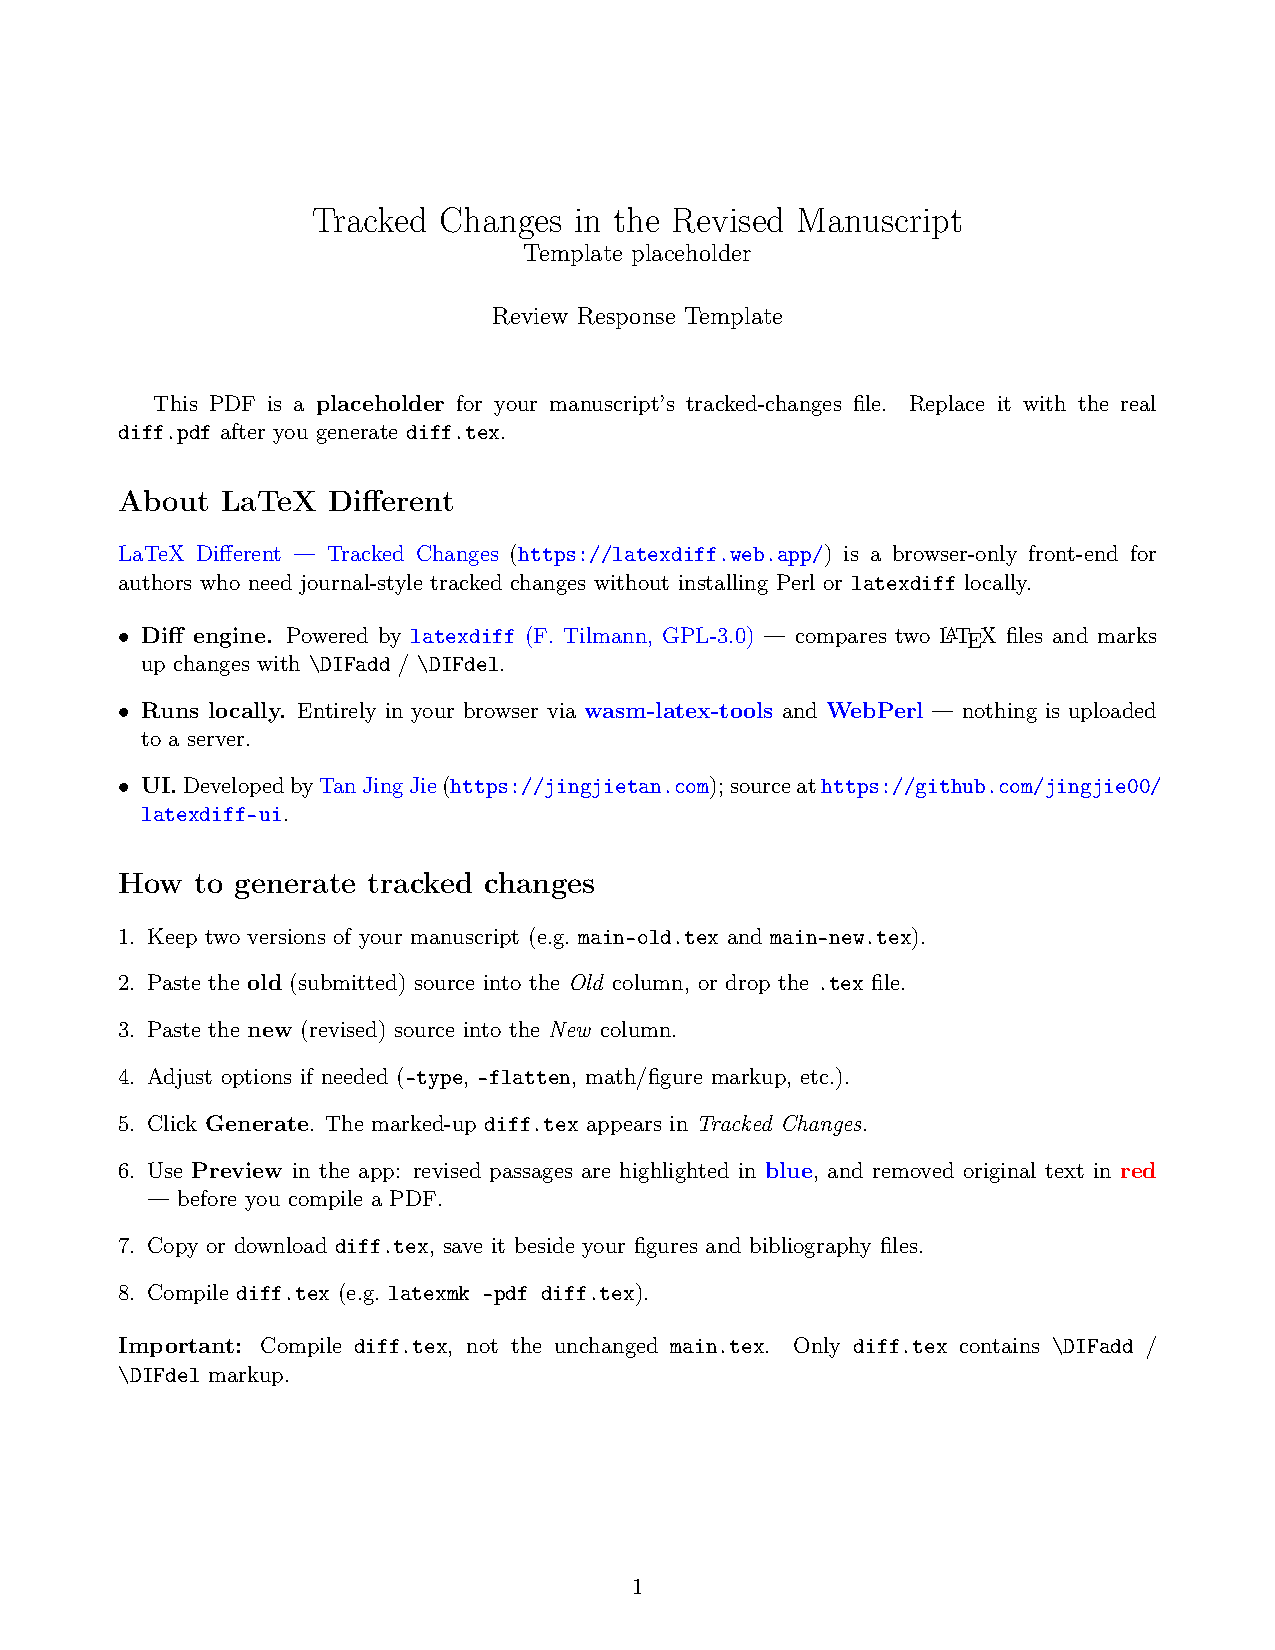
\includepdf[pages=-]{tracked-changes-guide.pdf}

\end{document}
